% paper/sections/13e2_ao_capillary_split_gate.tex
%
% V11: active-geometry capillary split integration gate
% ═══════════════════════════════════════════════════════════════════════════════
\subsection{V11：アクティブ幾何毛管分解の統合ゲート}
\label{sec:ao_fast_capillary_gate}

\paragraph{目的．}
V11 は U12 の代数診断を，第~\ref{sec:verification}章の統合検証文脈へ接続するゲートである．
U12 が棄却したのは，全セル圧力像へ毛管仕事を過射影して
非静的波の駆動まで消す古い分解である．
V11 では，その反例を踏まえて，
式~\eqref{eq:capillary_pressure_reaction_projection} の $R_p$，
式~\eqref{eq:ao_projection_face_bridge} の Hodge 逆適用済み面補間，
式~\eqref{eq:ao_graph_hfe_jump}--\eqref{eq:ao_graph_hfe_face_law} の
$q$ 所有グラフ HFE 圧力ジャンプ，
式~\eqref{eq:ao_face_cochain_regrid} の移動格子面共鎖移送，
式~\eqref{eq:ao_pressure_coordinate_split} の滑らかな圧力履歴座標，
式~\eqref{eq:ao_dc_convergence_gate} の DC 収束判定，
および式~\eqref{eq:grid_regular_stratum_axis}--\eqref{eq:grid_regular_stratum_shift}
の正則層ガードを
同時に満たすことを，アクティブ幾何毛管分解の統合条件として固定する．

\paragraph{検査項目．}
V11 は以下を同時に要求する．
\begin{enumerate}[noitemsep]
  \item 平坦・静的ゲート：平坦界面および静的平衡では
        $a_{\sigma,\mathrm{bal}}$ が丸め誤差まで $0$ になる．
  \item 毛管波ゲート：毛管波では，全圧力像ではなく
        物理的に許容される $R_p$ を用いた
        $r_\sigma-\Pi^{M_f}_{R_p}r_\sigma$ が非零の復元向き仕事を持つ．
  \item 精度ゲート：近似分解を用いる場合は式~\eqref{eq:ao_fast_error_budget} の
        共変量誤差と射影誤差を満たす．
  \item 面 Hodge ゲート：毛管共変量は式~\eqref{eq:ao_hodge_divided_face_increment}
        で一度だけ面加速度へ写し，投影面空間へは
        式~\eqref{eq:ao_projection_face_bridge} の同次元補間で渡す．
  \item グラフ HFE ゲート：柱状高さグラフでは
        式~\eqref{eq:ao_graph_hfe_cut} の現在グラフで HFE を切り，
        式~\eqref{eq:ao_graph_hfe_jump} のジャンプを現在格子の face law として使う．
  \item 移動格子ゲート：投影済み面共鎖を節点速度補間で作り直さず，
        新格子の Hodge 計量へ移送する．
  \item 正則層ゲート：追随格子の節点退避は
        最大 $|\partial_a\phi|$ の座標方向だけで行い，界面接線方向の
        格子幅を壊さない．
  \item 履歴・収束ゲート：圧力履歴は滑らかな座標だけを保存し，
        幾何毛管反力は現在段階の反力として扱い，DC は収束判定で受理する．
\end{enumerate}

\begin{table}[htbp]
\caption{V11：アクティブ幾何毛管分解の統合ゲート判定}
\label{tab:V11_ao_gate}
\centering
\PaperTableDenseSetup
\begin{tabularx}{\linewidth}{@{}>{\raggedright\arraybackslash}p{0.22\linewidth}>{\raggedright\arraybackslash}X>{\raggedright\arraybackslash}p{0.18\linewidth}@{}}
\toprule
項目 & 観測と解釈 & 判定 \\
\midrule
平坦・静的ゲート & 平坦界面はゼロ駆動．静的問題で非零駆動を作る経路は標準経路へ入れない． & \checkmark \\
全圧力像の反例 & N32/N64 毛管波で厳密全圧力分解は釣合い駆動を $0$ にする．これは成功ではなく過射影の反例である． & \checkmark 診断 \\
成分体積 Hodge 診断 & 同じ毛管波で成分体積 Hodge 診断は N32/N64 の釣合いノルム $2.1176/2.3055$ を検出する．ただしこれは最終 $R_p$ の代替証明ではなく非静的性の診断である． & \checkmark 診断 \\
$q$ 所有グラフ HFE & 圧力ジャンプは $j_{gl}^{G}=-(\sigma/\Delta x_i)\partial S_G/\partial H_i$，切断面は $\psi_G=h_G(q)-y$．pressure-coordinate history へ不連続ジャンプを保存せず，現在格子で面ジャンプを再構築する． & \checkmark 契約 \\
追随格子正則層 & 620 step 診断で支配法線方向ガードにより $\Delta x_{\min}=6.25\times10^{-4}\,\mathrm{m}$ を保持し，PPE RHS は $\Ord{10^4}$ に留まった．全 active 軸移動で見られた接線方向格子崩壊は再現しない． & \checkmark \\
1 周期統合走行 & 第~\ref{sec:val_capillary}節の N32 毛管波は $T_\sigma=0.046742983863\,\mathrm{s}$ まで完走し，体積ドリフト最大 $4.66\times10^{-14}$，運動エネルギー最大 $8.32\times10^{-6}$，終端振幅比 $0.794$ を得た． & \checkmark 物理ベンチへ接続 \\
最終採用境界 & $R_p$，Hodge 逆適用済み面補間，$q$ 所有グラフ HFE，移動格子面共鎖，圧力履歴座標，正則層ガード，DC 収束判定を同時に満たす経路だけをアクティブ幾何毛管分解として標準物理経路へ入れる． & \checkmark 契約 \\
\bottomrule
\end{tabularx}
\end{table}

\begin{figure}[htbp]
\centering
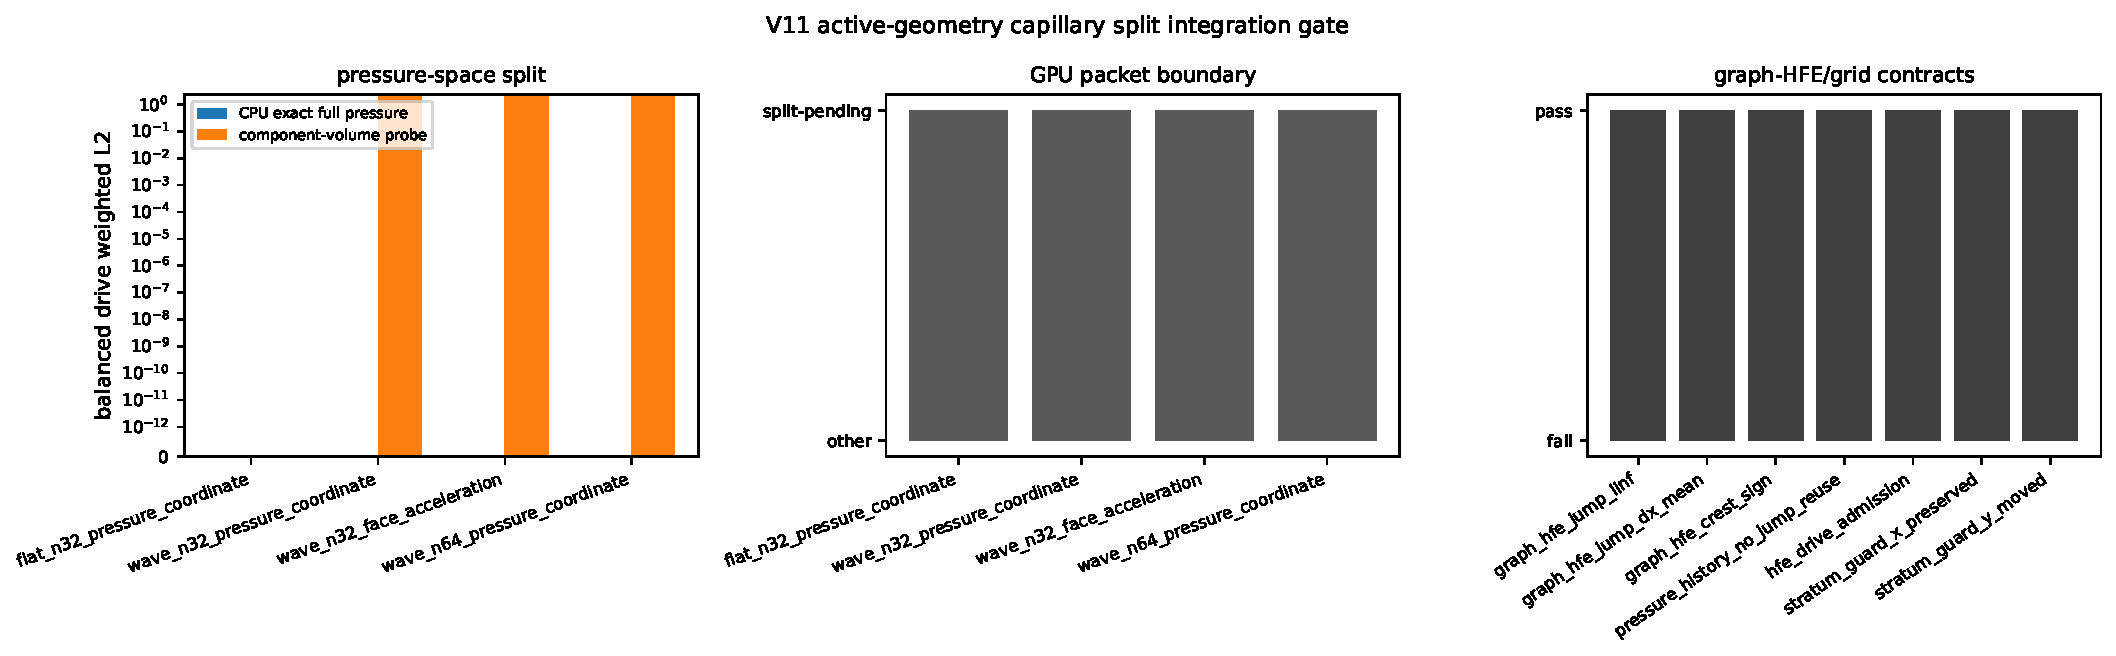
\includegraphics[width=0.78\linewidth]{figures/ch13_v11_ao_capillary_split_gate.pdf}
\caption{V11：アクティブ幾何毛管分解の統合ゲート．
圧力座標と面加速度の履歴表現を含め，
非静的波では全圧力像への過射影を棄却し，最終 $R_p$ 契約へ進めることを確認する．}
\label{fig:V11_ao_gate}
\end{figure}

\paragraph{第14章への接続．}
V11 は，過射影で非静的駆動を消す古い分解を棄却し，
第~\ref{sec:ao_fast_state_space}節の採用条件を本番経路の境界として固定する．
したがって第~\ref{sec:val_capillary}節の毛管波は，
幾何セル分率，bundle Young--Laplace work，pressure-component Hodge reaction，
Hodge 逆適用済み面補間，$q$ 所有グラフ HFE，投影済み面共鎖保存，
正則層ガード，および pressure-coordinate history を同時に使う
アクティブ幾何毛管分解の物理ベンチマークとして読む．
ただし，U12 が棄却した全圧力像への過射影や，
面共鎖移送を欠く節点速度再構成経路は，本節の合格経路ではない．
